\documentclass[tikz,border=2pt]{standalone}
\usepackage{amsmath,amssymb}
\usetikzlibrary{arrows.meta}

\begin{document}
% Deleted infinite broom: the segments from the origin to (1, 1/n), n = 1, 2, ..., together with
% the single point (1, 0). The segment from the origin to (1, 0) itself is not part of the set.
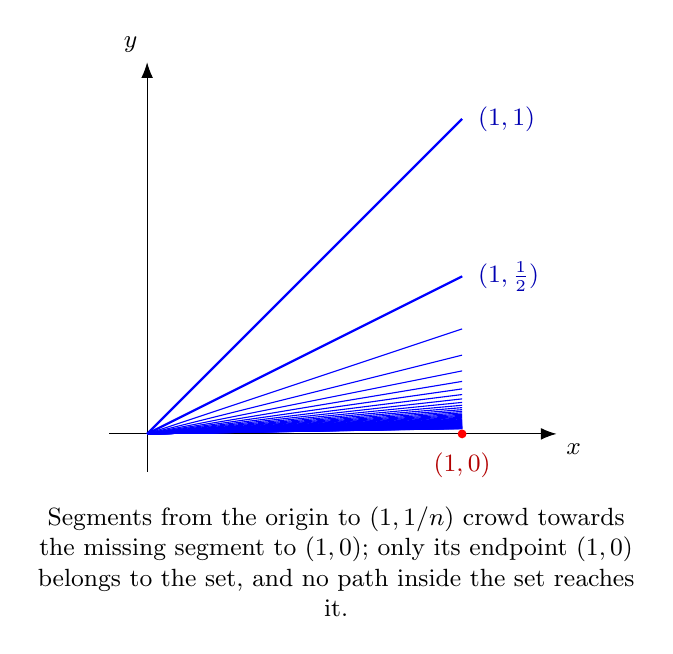
\begin{tikzpicture}[every node/.style={font=\small}, >={Latex[length=2mm]}, x=4cm, y=4cm]
	\draw[->] (-0.12,0) -- (1.3,0) node[below right] {$x$};
	\draw[->] (0,-0.12) -- (0,1.18) node[above left] {$y$};
	\foreach \n in {1,...,60} {
		\draw[blue, thin] (0,0) -- (1,1/\n);
	}
	\draw[blue, thick] (0,0) -- (1,1);
	\draw[blue, thick] (0,0) -- (1,1/2);
	\fill[red] (1,0) circle (1.6pt);
	\node[red!70!black, anchor=north, font=\small] at (1,-0.03) {$(1,0)$};
	\node[blue!70!black, anchor=west, font=\small] at (1.02,1) {$(1,1)$};
	\node[blue!70!black, anchor=west, font=\small] at (1.02,0.5) {$(1,\tfrac12)$};
	\node[anchor=north, align=flush center, text width=7.6cm] at (0.6,-0.2) {Segments from the origin to $(1,1/n)$ crowd towards the missing segment to $(1,0)$; only its endpoint $(1,0)$ belongs to the set, and no path inside the set reaches it.};
\end{tikzpicture}
\end{document}
